\section{Program Sampling}
\label{sec:program-sampling}
The search space an algorithm explores determines the best programs it can find.
The considered search spaces in existing approaches are limited by the following factors: (1) Manual enumeration (\textit{e.g.}, TVM \cite{chen2018learning}). It is impractical to manually enumerate all possible choices by templates, so existing manual templates only cover a limited search space heuristically. (2) Aggressive early pruning (\textit{e.g.}, Halide auto-scheduler \cite{adams2019learning}). Aggressive early pruning based on evaluating incomplete programs prevents the search algorithm from exploring certain regions in the space.

In this section, we introduce techniques to push the boundary of the considered search space by addressing the above limitations. To solve (1), we automatically expand the search space by recursively applying a set of flexible derivation rules. To avoid (2), we randomly sample complete programs in the search space.
Since random sampling gives an equal chance to every point to be sampled, our search algorithm can potentially explore every program in the considered space.
We do not rely on random sampling to find the optimal program, because every sampled program is later fined-tuned (\autoref{sec:performance-fine-tuning}).



\begin{table*}[t!]
	\renewcommand{\arraystretch}{1.2}
	\footnotesize
	\centering
	\begin{tabular}{llll}
		\hline
		No & Rule Name & Condition & Application  \\
		\hline
		1 & Skip &  $\neg  IsStrictInlinable(S, i)$  & $S' = S;  i' = i - 1$ \\
		2 & Always Inline  & $IsStrictInlinable(S, i) $  & $S' = Inline(S, i)$; $i' = i - 1$ \\
		3 & Multi-level Tiling & $HasDataReuse(S, i)$ & $S' = MultiLevelTiling(S, i); i' = i - 1$ \\
		4 & Multi-level Tiling with Fusion& $HasDataReuse(S, i) \wedge HasFusibleConsumer(S, i) $  & $S' = FuseConsumer(MultiLevelTiling(S, i),i); i' = i - 1$ \\
		5 & Add Cache Stage & $HasDataReuse(S, i) \wedge \neg HasFusibleConsumer(S, i) $  & $S' = AddCacheWrite(S, i); i = i' $ \\
		6 & Reduction Factorization &  $HasMoreReductionParallel(S, i)$ & $S' = AddRfactor(S, i); i' = i - 1 $  \\
		... & User Defined Rule &  ... & ...  \\
		\hline
	\end{tabular}
	\vskip -0.4em
	\caption{Derivation rules used to generate sketches. The condition runs on the current state $\sigma = (S, i)$. The application derives the next state $\sigma' = (S', i')$ from the current state $\sigma$. Note that some function (\textit{e.g.}, $AddRfactor$, $FuseConsumer$) can return multiple possible values of $S'$. In this case we collect all possible $S'$, and return multiple next states $\sigma'$ for a single input state $\sigma$.}
	\postcap
	\label{table:derivation-rules}
\end{table*}


To sample programs that can cover a large search space, we define a hierarchical search space with two levels: \textit{sketch} and \textit{annotation}.
We define the high-level structures of programs as sketches and leave billions of low-level choices (\textit{e.g.}, tile size, parallel, unroll annotations) as annotations.
At the top level, we generate sketches by recursively applying a few derivation rules.
At the bottom level, we randomly annotate these sketches to get complete programs.
This representation summarizes a few basic structures from billions of low-level choices, enabling the flexible enumeration of high-level structures and efficient sampling of low-level details.

While \Ansor supports both CPU and GPU, we explain the sampling process for CPUs in \autoref{subsec:sketch-generation} and \autoref{subsec:random-sampling} as an example.
We then discuss how the process is different for GPU in \autoref{subsec:gpu-support}.

\subsection{Sketch Generation}
\label{subsec:sketch-generation}
As shown in \autoref{fig:system-overview}, the program sampler accepts partitioned subgraphs as input.
The first column in \autoref{fig:sampled-program-examples} shows two examples of the input.
The input has three equivalent forms: the mathematical expression, the corresponding naive program obtained by directly expanding the loop indices, and the corresponding computational graph (directed acyclic graph, or DAG).

To generate sketches for a DAG with multiple nodes, we visit all the nodes in a topological order and build the structure iteratively.
For computation nodes that are compute-intensive and have a lot of data reuse opportunities (\textit{e.g.}, conv2d, matmul), we build basic tile and fusion structures for them as the sketch.
For simple element-wise nodes (\textit{e.g.}, ReLU, element-wise add), we can safely inline them.
Note that new nodes (\textit{e.g.}, caching nodes, layout transform nodes) may also be introduced to the DAG during the sketch generation.

We propose a derivation-based enumeration approach to generate all possible sketches by recursively applying several basic rules.
This process takes a DAG as an input and returns a list of sketches.
We define the State $\sigma = (S, i)$, where $S$ is the current partially generated sketch for the DAG, and $i$ is the index of the current working node.
The nodes in a DAG are sorted in a topological order from output to input.
The derivation begins from the initial naive program and the last node, or the initial state $\sigma = (naive\ program, index\ of \ the\ last\ node)$.
Then we try to apply all derivation rules to the states recursively.
For each rule, if the current state satisfies the application condition, we apply the rule to $\sigma = (S, i)$ and get $\sigma' = (S', i')$ where $i' \le i$.
This way the index $i$ (working node) decreases monotonically.
A state becomes a terminal state when $i = 0$.
During enumeration, multiple rules can be applied to one state to generate multiple succeeding states. One rule can also generate multiple possible succeeding states. So we maintain a queue to store all intermediate states. The process ends when the queue is empty.
All $\sigma.S$ in terminal states form a sketch list at the end of the sketch generation. The number of sketches is less than 10 for a typical subgraph.

\textbf{Derivation rules.}
\autoref{table:derivation-rules} lists derivation rules we used for the CPU.
We first provide the definition of the used predicates and then describe the functionality of each rule.
$IsStrictInliable(S, i)$ indicates if the node $i$ in $S$ is a simple element-wise operator that can always be inlined (\textit{e.g.}, element-wise add, ReLU). $HasDataReuse(S, i)$ indicates if the node $i$ in $S$ is a compute-intensive operator and has plentiful intra-operator data reuse opportunity (\textit{e.g.}, matmul, conv2d). $HasFusibleConsumer(S, i)$ indicates if the node $i$ in $S$ has only one consumer $j$ and node $j$ can be fused into node $i$ (\textit{e.g.}, matmul + bias\_add, conv2d + relu). $HasMoreReductionParallel(S, i)$ indicates if the node $i$ in $S$ has little parallelism in space dimensions but has ample parallelism opportunity in reduction dimensions.  (\textit{e.g.}, computing 2-norm of a matrix, matmul $C_{2\times 2} = A_{2\times 512} \cdot B_{512 \times 2}$).
We perform static analysis on the computation definitions to get the values for these predicates.
The analysis is done automatically by parsing the read/write pattern in the mathematical expressions.
Next, we introduce the functionality of each derivation rule.

Rule 1 just simply skips a node if it is not strictly inlinable. Rule 2 always inlines strictly inlinable nodes. Since the conditions of rule 1 and rule 2 are mutually exclusive, a state with $i>1$ can always satisfy one of them and continue to derive.

Rules 3, 4, and 5 deal with the multi-level tiling and fusion for nodes that have data reuse.
Rule 3 performs multi-level tiling for data reusable nodes. For CPU, we use a ``SSRSRS'' tile structure, where ``S'' stands for one tile level of space loops and ``R'' stands for one tile level of reduction loops. For example, in the matmul $C(i, j) = \sum_k A[i,k] \times B[k, j]$, $i$ and $j$ are space loops and $k$ is a reduction loop. The ``SSRSRS'' tile structure for matmul expands the original 3-level loop $(i, j, k)$ into a 10-level loop $(i_0, j_0, i_1, j_1, k_0, i_2, j_2, k_1, i_3, j_3)$. Although we do not permute the loop order, this multi-level tiling can also cover some cases of reordering.
For example, the above 10-level loop can be specialized to just a simple reorder $(k_0, j_2, i_3)$ by setting the length of other loops to one.
The "SSRSRS" tile structure is general for compute-intensive dense operators (\textit{e.g.}, matmul, conv2d, conv3d) in deep learning, because they all consist of space loops and reduction loops.

Rule 4 performs multi-level tiling and also fuses the fusible consumers. For example, we fuse the element-wise nodes (\textit{e.g.}, ReLU, bias add) into the tiled nodes (\textit{e.g.}, conv2d, matmul).
Rule 5 adds a caching node if the current data-reusable node does not have a fusible consumer.
For example, the final output node in a DAG does not have any consumer, so it directly writes results into main memory by default and this is inefficient due to the high latency of memory accesses.
By adding a cache node, we introduce a new fusible consumer into the DAG, then rule 4 can be applied to fuse this newly added cache node into the final output node.
With the cache node fused, now the final output node writes its results into a cache block, and the cache block will be written to the main memory at once when all data in the block is computed.

Rule 6 can use \texttt{rfactor} \cite{suriana2017parallel} to factorize a reduction loop into a space loop to bring more parallelism.


\begin{figure*}[t!]
	\centering
	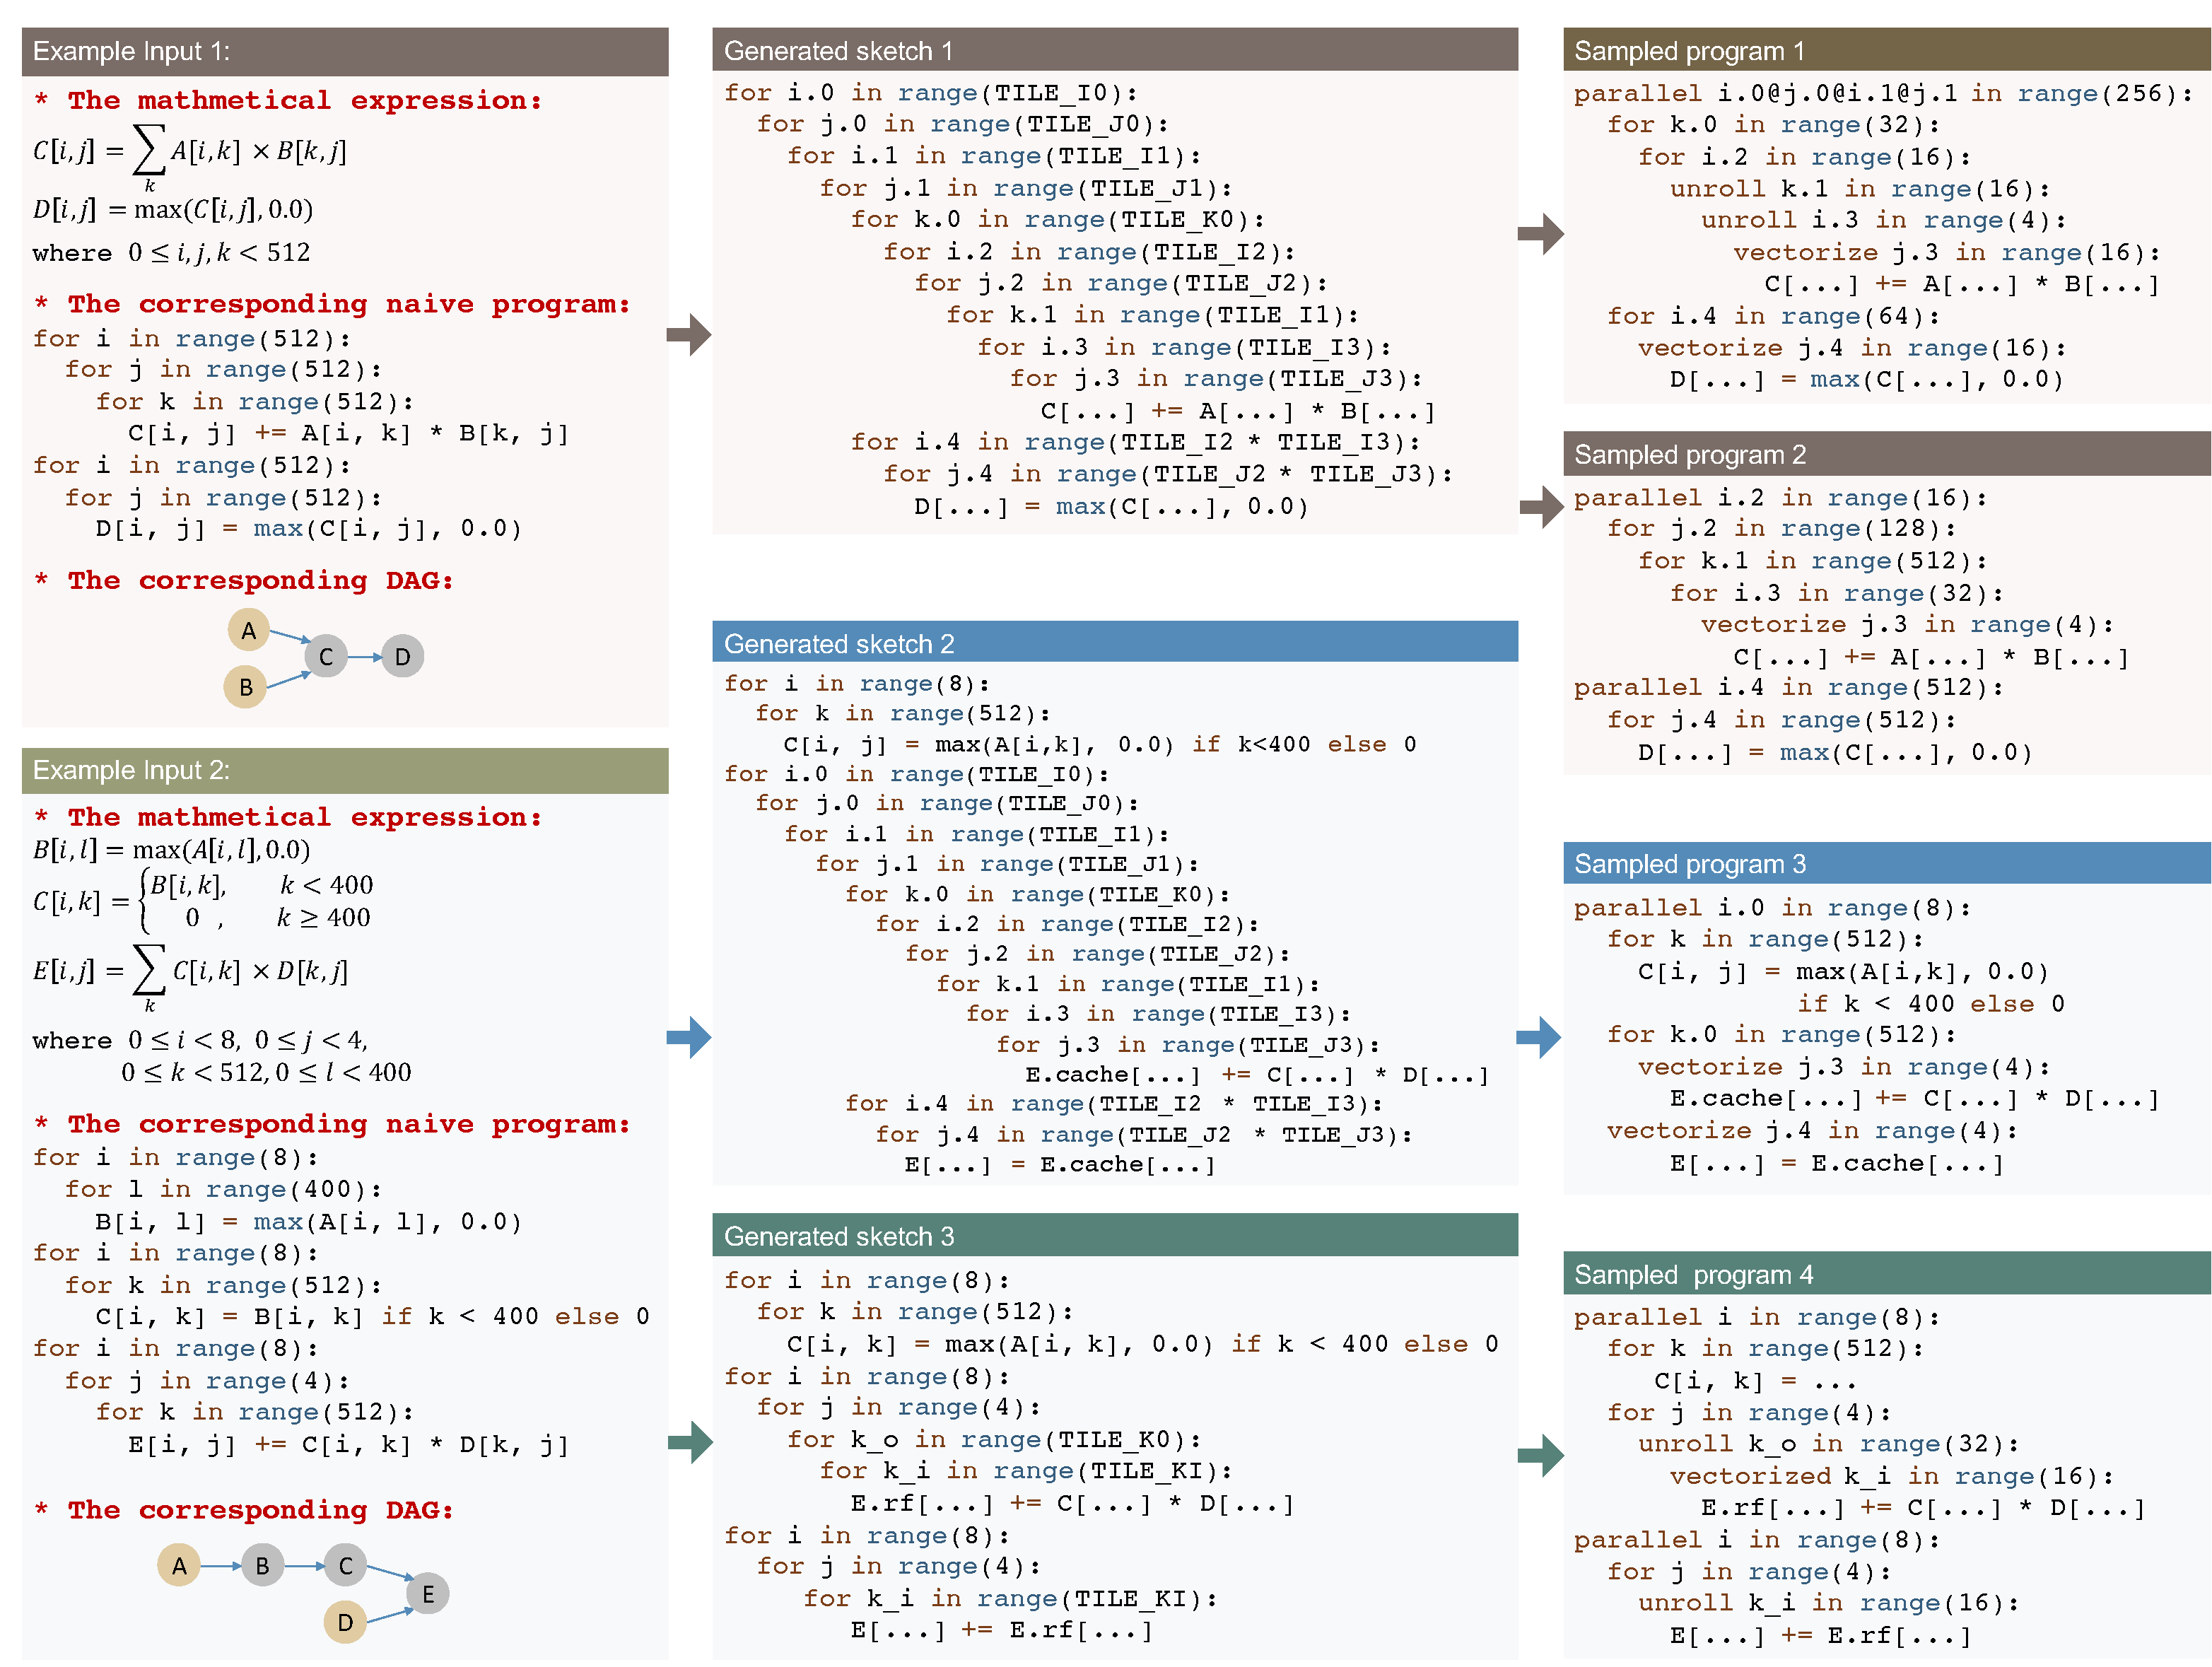
\includegraphics[width=\textwidth]{figures/sampled-program-examples.pdf}
	\vskip -0.8em
	\caption{Examples of generated sketches and sampled programs. This figure shows two example inputs, three generated sketches and four sampled programs. The code example is pseudo code in a python-like syntax.}
	\postcap
	\label{fig:sampled-program-examples}
\end{figure*}

\textbf{Examples.}
\autoref{fig:sampled-program-examples} shows three examples of the generated sketches.
The sketches are different from the manual templates in TVM, because the manual templates specify both high-level structures and low-level details while sketches only define high-level structures.
For the example input 1, the sorted order of the four nodes in the DAG is $(A, B, C, D)$.
To derive the sketches for the DAG, we start from output node $D (i=4)$ and apply rules to the nodes one by one.
Specifically, the derivation for generated sketch 1 is:
\preeq \preeq \preeq
\begin{align*}
Input~1  \rightarrow  & \sigma(S_0, i = 4)  \xrightarrow{\text{Rule 1}}  \sigma(S_1, i = 3)  \xrightarrow{\text{Rule 4}}  \\ 
 & \sigma(S_2, i = 2)   \xrightarrow{\text{Rule 1}}  \sigma(S_3, i = 1)  \xrightarrow{\text{Rule 1}}  Sketch~1
\end{align*}
\posteq

For the example input 2, the sorted order of the five nodes is $(A, B, C, D, E)$.
Similarly, we start from the output node $E (i=5)$ and apply rules recursively.
The generated sketch 2 is derived by:
\preeq \preeq \preeq
\begin{align*}
 Input~2 \rightarrow  & \sigma(S_0, i = 5)  \xrightarrow{\text{Rule 5}}  \sigma(S_1, i = 5)  \xrightarrow{\text{Rule 4}} \\
 & \sigma(S_2, i = 4)  \xrightarrow{\text{Rule 1}} \sigma(S_3, i = 3) \xrightarrow{\text{Rule 1}} \\
 & \sigma(S_4, i = 2)  \xrightarrow{\text{Rule 2}} \sigma(S_5, i = 1)  \xrightarrow{\text{Rule 1}}  Sketch~2
\end{align*}
\posteq

\noindent Similarly, the generated sketch 3 is derived by:

\preeq \preeq
\begin{align*}
Input~2 \rightarrow  & \sigma(S_0, i = 5)  \xrightarrow{\text{Rule 6}}  \sigma(S_1, i = 4)  \xrightarrow{\text{Rule 1}} \\
& \sigma(S_2, i = 3)  \xrightarrow{\text{Rule 1}} \sigma(S_3, i = 2) \xrightarrow{\text{Rule 2}} \\
& \sigma(S_4, i = 1)  \xrightarrow{\text{Rule 1}}  Sketch~3
\end{align*}
\posteq


\textbf{Customization.}
While the presented rules are practical enough to cover the structures for most operators, there are always exceptions.
For example, some special algorithms (\textit{e.g.}, Winograd convolution~\cite{lavin2016fast}) and accelerator intrinsics (\textit{e.g.}, TensorCore~\cite{nvidia2017tensorcore}) require special tile structures to be effective.
Although the template-guided search approach (in TVM) can craft a new template for every new case, it needs a great amount of design effort.
On the other hand, the derivation-based sketch generation in \Ansor is flexible enough to generate the required structures for emerging algorithms and hardware, as we allow users to register new derivation rules and integrate them seamlessly with existing rules.

\subsection{Random Annotation}
\label{subsec:random-sampling}

The sketches generated by the previous subsection are incomplete programs because they only have tile structures without specific tile sizes and loop annotations, such as parallel, unroll, and vectorization.
In this subsection, we annotate sketches to make them complete programs for fine-tuning and evaluation.

Given a list of generated sketches, we randomly pick one sketch, randomly fill out tile sizes, parallelize some outer loops, vectorize some inner loops, and unroll a few inner loops.
We also randomly change the computation location of some nodes in the program to make a slight tweak to the tile structure.
All ``random'' in this subsection means a uniform distribution over all valid values.
If some special algorithms require custom annotations to be effective (\textit{e.g.}, special unrolling), we allow users to give simple hints in the computation definition to adjust the annotation policy.
Finally, since changing the layout of constant tensors can be done in compilation time and brings no runtime overhead, we rewrite the layouts of the constant tensors according to the multi-level tile structure to make them as cache-friendly as possible.
This optimization is effective because the weight tensors of convolution or dense layers are constants for inference applications.

Examples of random sampling are shown in \autoref{fig:sampled-program-examples}.
The sampled program might have fewer loops than the sketch because the loops with length one are simplified.

\subsection{GPU Support}
\label{subsec:gpu-support}

For GPU, we change the  multi-level tiling structure from "SSRSRS" to "SSSRRSRS" to match the architecture of GPU. The loops in the first three space tiles are bound to BlockIdx, virtual thread (for reducing bank conflicts), and ThreadIdx, respectively. We add two sketch derivation rules, one for utilizing shared memory by inserting a caching node (similar to Rule 5) and the other for cross-thread reduction (similar to Rule 6).


